% ==========================================
% Technical Report - Equalizer ( hullb2 )
% ==========================================
\chapter{Equalizer}

\section{Introduction}
Equalizer is an \gls{api} for creating parallel applications based on \gls{opengl}. It allows the creation of scalable graphics applications. Furthermore, these applications can be run unmodified on any multipipe visualisation system such as laptops, workstations, multipipe shared memory system or even graphic clusters. 

The framework Equalizer is available as open source under the \gls{lgpl} license. Furthermore, it runs on Linux, Windows XP and Mac OS X systems. It supports both 32-bit and 64-bit architecture.

This chapter gives an introduction to Equalizer and how it was used in this project. Used Equalizer graphics are by courtesy of Stefan Eilemann, Equalizer developer.

\section{Purpose of Equalizer}
There are two main motivations for parallelising the rendering.

\begin{description}
	\item[Multi-View Rendering] \hfill\\To run an application on systems with multiple displays - so called multipipe display systems. This includes workstations with multiple monitors or projectors as well as immersive environments such as a \gls{cave} or head mounted displays. Immersive environments additionally require active or passive stereo rendering. \\Multi-View rendering requires the synchronisation of the output of the different displays in order to provide one coherent image.
	\item[Scalable Rendering] \hfill\\To run an application that hits the limitations of a single graphics system due to the hardware. The rendering can be accelerated by aggregating multiple resources.
\end{description}

Equalizer provides methods to satisfy both of these motivations and they are not even mutually exclusive. This makes Equalizer a very powerful and flexible framework.

There are other existing generic approaches for parallelising rendering. A well-known solutions is Chromium, which was originally developed at the Stanford University. Like Equalizer, it enables applications to use multiple graphics cards for rendering. But other than Equalizer, Chromium is focused on streaming the \gls{opengl} commands through a network of nodes, often initiated from a single server. These \gls{opengl} streams can be very large if they contain texture images in addition to the \gls{opengl} commands. This is a major limitation and often leads to the fact that the network is the performance bottleneck.

To get rid of this problem, Equalizer follows a different approach for rendering. It runs the application, of which each client in the network has a copy, in parallel and uses the network only for synchronisation. 

The main features, that characterise Equalizer are:
\begin{itemize}
\item Runtime Configurability
\item Runtime Scalability
\item Distributed Execution
\item Support for Stereo and Immersive Environments
\end{itemize}

The following table shows the main differences between Equalizer and Chromium:

\begin{table}[H]
\centering
\begin{tabular}{|p{0.4\textwidth}|p{0.4\textwidth}|}
	\hline
	\bfseries Transparent Layer: Chromium & \bfseries Parallel \gls{api}: Equalizer \\
	\hline
	\hline 
	runs unmodified applications & minimally invasive API: application has to be adapted \\
	\hline
	focus on transparency for applications & focus on parallel rendering performance and scalability \\
	\hline
	operates on \gls{opengl} command stream & parallelises application \\
	\hline
	single application rendering thread & multithreaded and potentially distributed application \\
	\hline
	mostly used for rendering to multiple, planar displays, immersive installations may require application changes & multi-display and immersive installations, many-to-one scalable rendering \\
	\hline
	limited \gls{opengl} extension support and compatibility & full \gls{opengl} compatibility: does not interfere with \gls{opengl} rendering code \\
	\hline
\end{tabular}
\caption{Chromium vs. Equalizer\cite{website:equalizer}}
\end{table}

Figure \ref{fig:eqVsChromium} visualises the different approaches of Chromium and Equalizer. Chromium streams the \gls{opengl} calls to the clients as shown in figure \ref{fig:eqVsChromium} (c) whereas Equalizer runs parts of the application in parallel on multiple rendering clients \ref{fig:eqVsChromium} (a).

\begin{figure}[H]
	\centering
	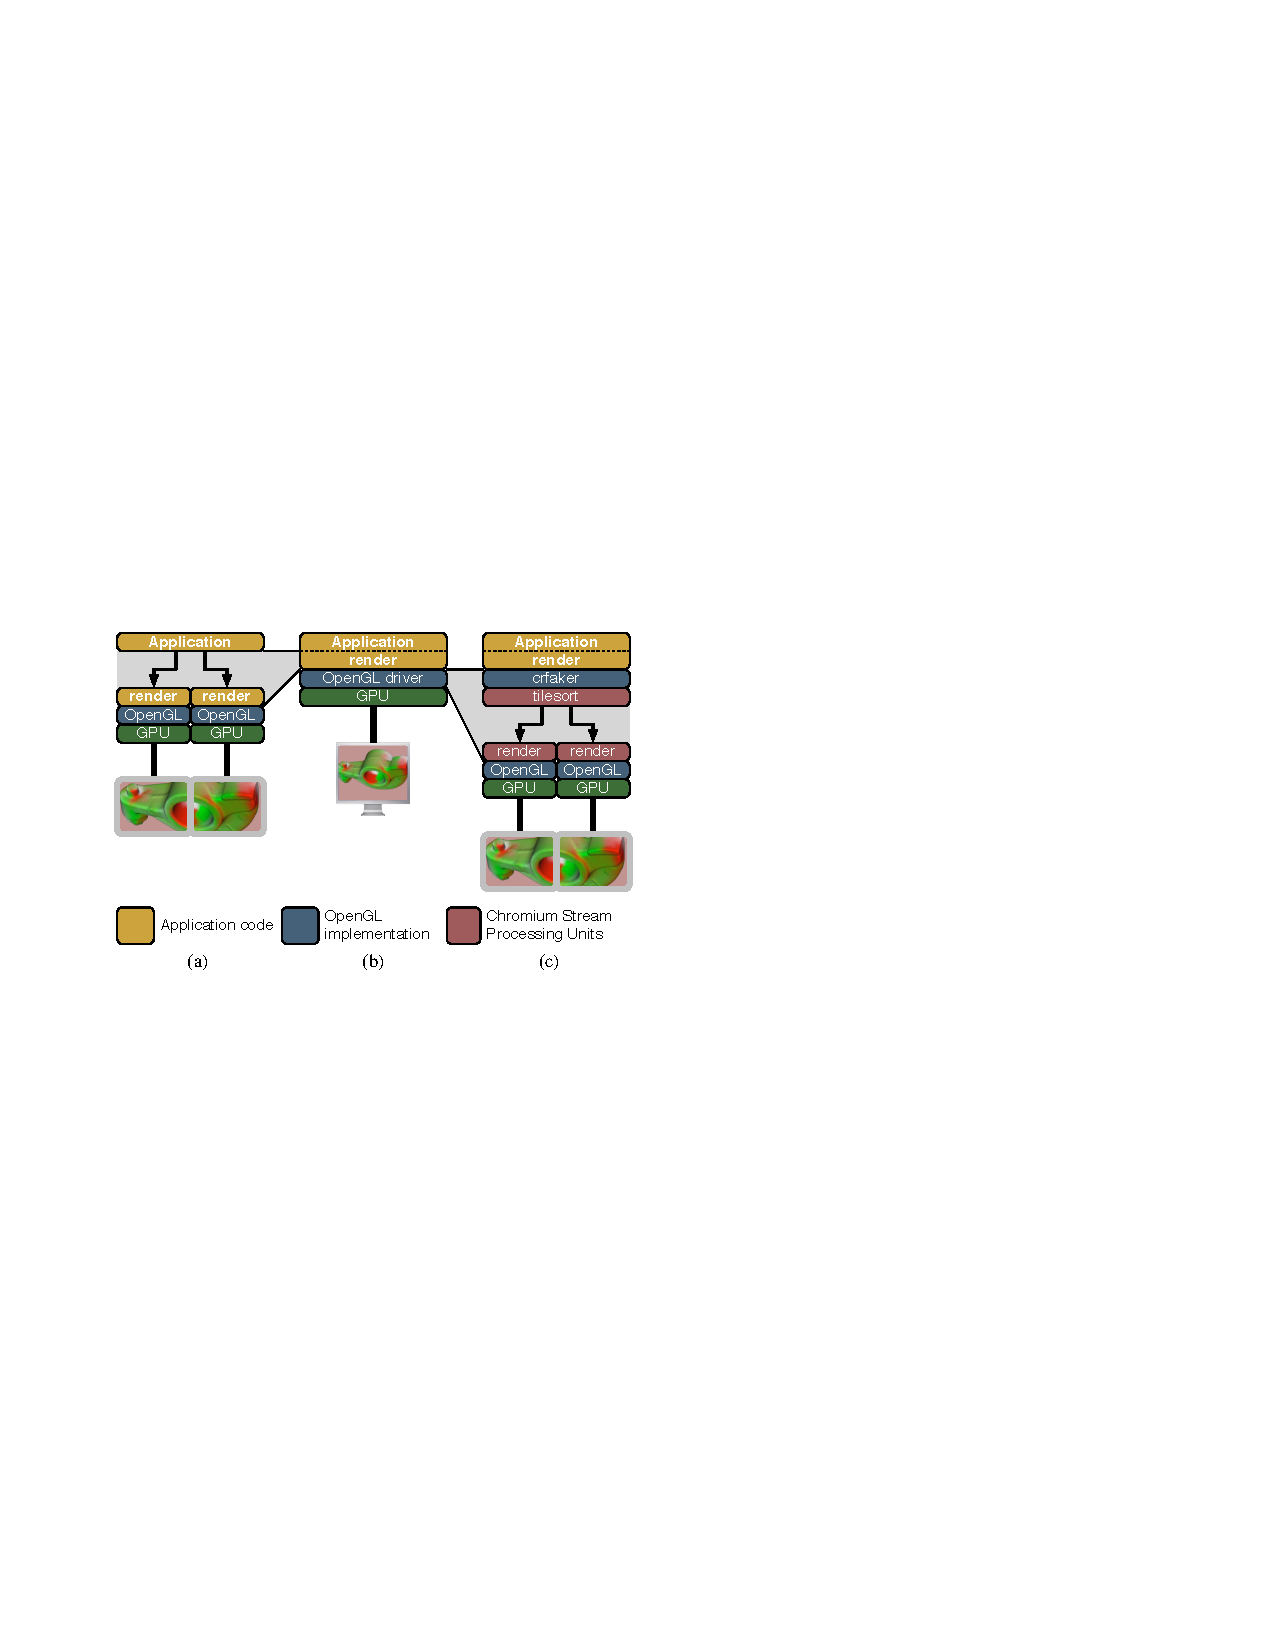
\includegraphics[width=0.6\textwidth]{../figures/eqVsChromium}
	\caption{A traditional OpenGL application (b) and its equivalents when using Equalizer (a) or Chromium(c)\cite{eqParallel}}
	\label{fig:eqVsChromium}
\end{figure}

\section{Basic Concepts of Equalizer}
Equalizer runs parts of the application in parallel on multiple rendering clients. A typical \gls{opengl} application has an event loop which is responsible for performing updates and redrawing the scene. To parallelise the event loop, one has to separate the rendering code from the main event loop. After that, the rendering code can be executed in parallel on different resources. This is the technique applied in Equalizer. Figure \ref{fig:eqParallelisation} visualises the concept.

\begin{figure}[H]
	\centering
	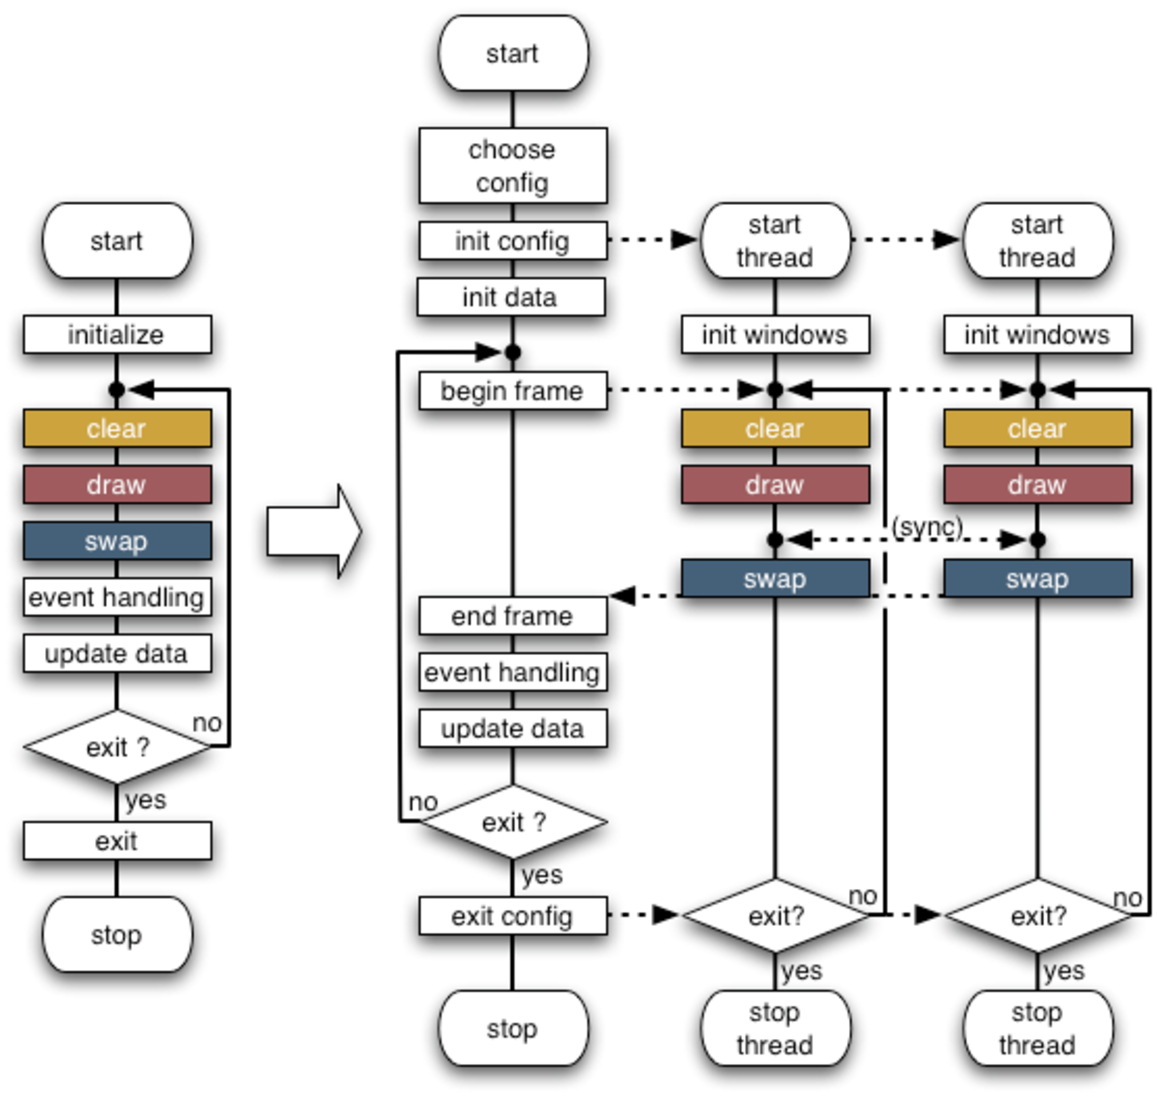
\includegraphics[width=0.5\textwidth]{../figures/parallel_rendering_execution_flow}
	\caption{Parallelised rendering pipeline as used in Equalizer\cite{website:equalizer}}
	\label{fig:eqParallelisation}
\end{figure}

Equalizer is based on a client-server model as shown in figure \ref{fig:eqClientServerModel}. The different parts and their responsibilities are discussed in detail in the following section:
\begin{description}
	\item[Server] \hfill\\The Equalizer server is responsible for one single visualisation system. It launches and controls the rendering clients of an application. It is only possible to run one application on a server at a time\footnote{In future releases of Equalizer, it should be possible to run multiple applications on one server.}.
	\item[Application] \hfill\\The application connects itself to an Equalizer server to receive a configuration. Furthermore, it provides render clients to the Equalizer server, which is responsible to control them. The application itself handles events (and updates data changes caused by events) and controls the rendering.
	\item[Render Clients] \hfill\\A render client implements the rendering part of the application. A render client has no main loop and is therefore completely driven by the Equalizer server. 
\end{description}

\begin{figure}[H]
	\centering
	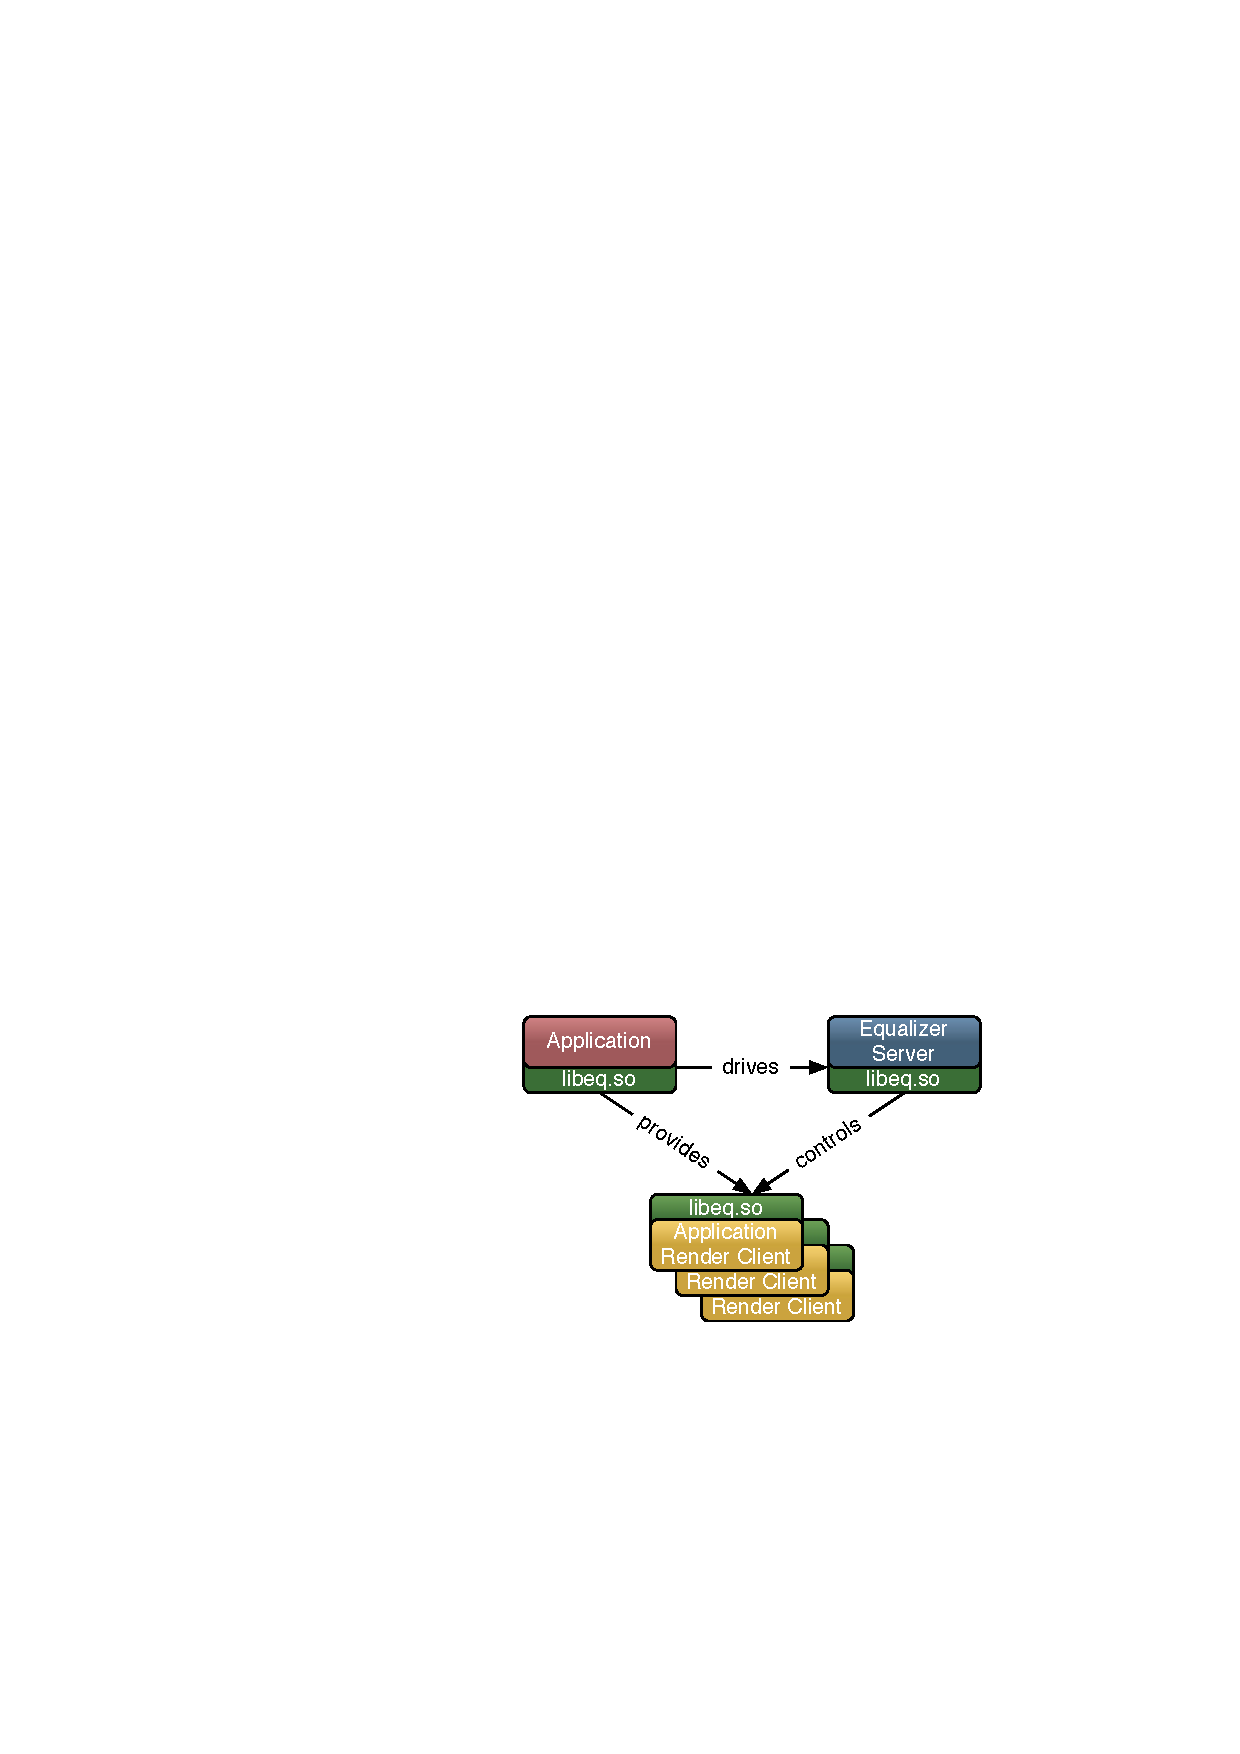
\includegraphics[width=0.5\textwidth]{../figures/eqClientServerModel}
	\caption{Client Server model of Equalizer\cite[p. 2]{eqPG}}
	\label{fig:eqClientServerModel}
\end{figure}

Figure \ref{fig:executionModel}\cite{eqPG} shows a simplified execution model and visualises how the described components of the Equalizer architecture work together.

\begin{figure}[H]
	\centering
	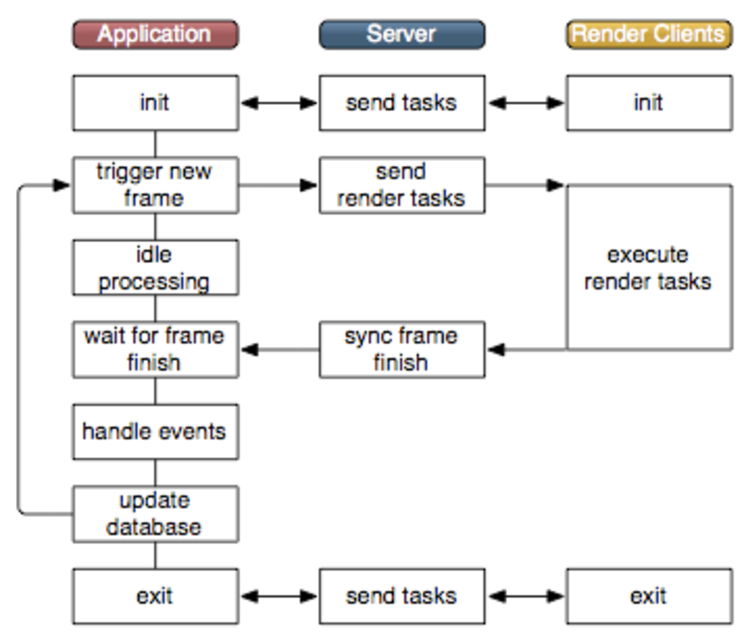
\includegraphics[width=0.5\textwidth]{../figures/equalizer_execution_flow}
	\caption{Simplified execution model of Equalizer\cite[p. 9]{eqPG}}
	\label{fig:executionModel}
\end{figure}

\subsection{Configurability}
\label{sec:configurability}
One of the major benefits of Equalizer is the flexible and scalable configuration of the parallel rendering tasks. An Equalizer configuration always uses a configuration server that allocates and balances the available resources. The server is configured using a hierarchically structured configuration file to describe the available resources and the combination of them for rendering. The structure in the configuration file has to correspond to the physical and logical topology. Equalizer introduces abstract components to describe the rendering resources and their relationship. The following list shows a collection of relevant components for this project. A complete list can be found in the Equalizer Programming Guide \cite[p. 55ff]{eqPG}.

\begin{description}
	\item[node] \hfill\\A node represents a single computer in a cluster. Equalizer handles each node as one operating system process of the rendering client. Nodes communicate with each other using \emph{connections}.
	\item[pipe] \hfill\\A \emph{pipe} is an abstraction of a graphics card (GPU). There may be multiple pipes per node.
	\item[window] \hfill\\A \emph{window} represents an \gls{opengl} drawable.
	\item[channel] \hfill\\A \emph{channel} stands for a viewport within a \emph{window}.
	\item[connection] \hfill\\A \emph{connection} is a stream-oriented point-to-point connection between nodes. Nodes either communicate other TCP/IP or SDP.
\end{description}

The configuration for the multiview rendering resources is defined through a compound tree with the following possible components:

\begin{description}
	\item[channel] \hfill\\Each compound has one channel which is used by the compound to execute the rendering task. A channel may be used by more than one compound.
	\item[frustum] \hfill\\Compounds have a frustum description to define the physical layout of the display environment. A frustum can be either a \emph{wall}\footnote{defined by the bottom-left, bottom-right and top-left edge coordinates} or a \emph{projection}\footnote{defined by the position and the head-pitch-roll orientation}.
	\item[attributes] \hfill\\Compounds have attributes to configure the decomposition of the destination channel's rendering.
\end{description}

Consult the Equalizer Programming Guide\cite{eqPG} for a detailed description of all configuration options.

Figure \ref{fig:eqSampleConfig} shows an example configuration. The left side of the tree defines the rendering resources and the right side defines the visualisation system which is a four sided \gls{cave} in this case. As one can see, it is possible to combine almost any resources. The matching between the rendering resources and the visualisation output is done via the \emph{channel} identifier. It is necessary to use unique descriptions for the \emph{name} of each channel.

\begin{figure}[H]
	\centering
	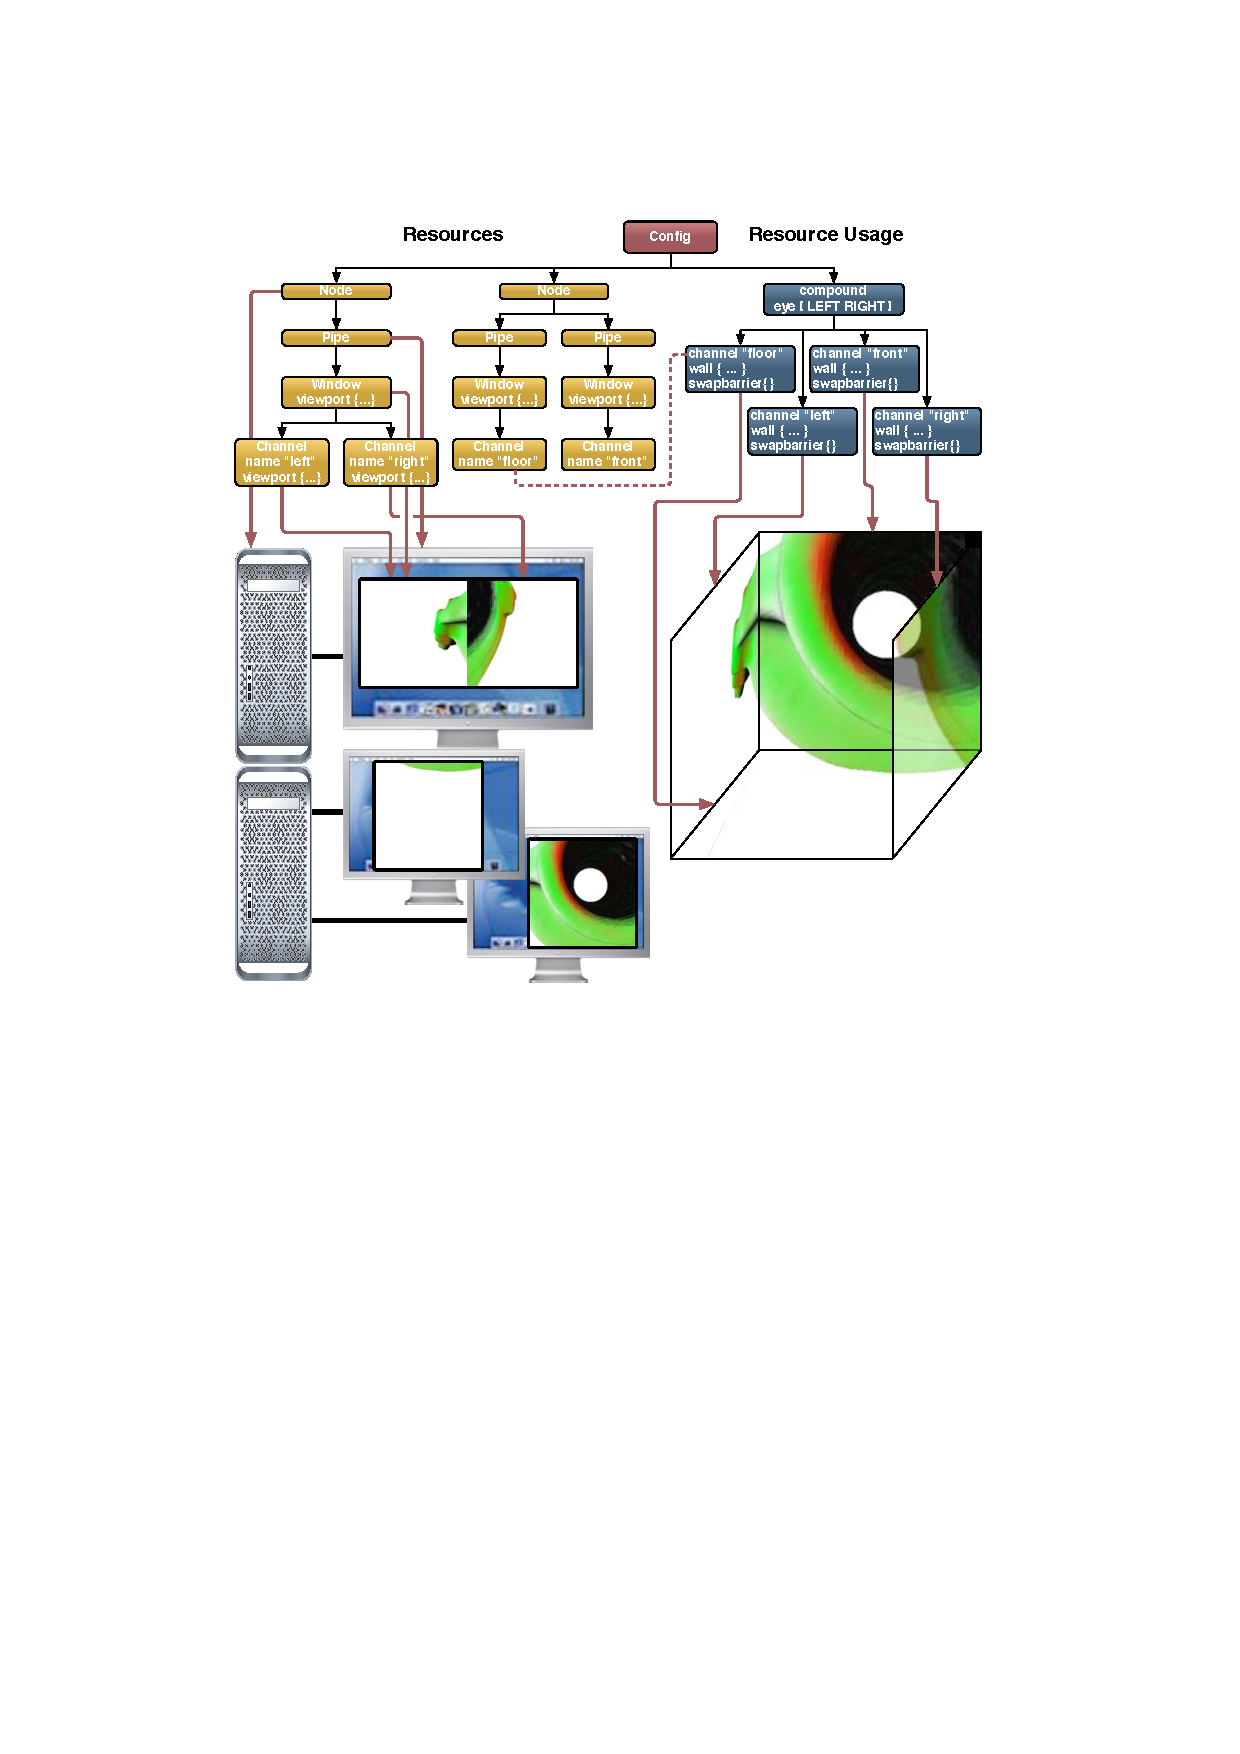
\includegraphics[width=0.8\textwidth]{../figures/eqSampleConfig}
	\caption{Example Configuration for a 4-sided CAVE\cite[p. 10]{eqPG}}
	\label{fig:eqSampleConfig}
\end{figure}

\subsection{Scalability}
Equalizer provides numerous scalability algorithms. Therefore, an application built with Equalizer is inherently scalable. The used algorithm for decomposition and composition can be configured through the Equalizer configuration file. The only thing the programmer has to ensure is that the critical parts of the application (the rendering code) are encapsulated. The rendering code itself can basically be retained. The only thing that has to be changed in the application code is that the application rendering code uses the frustum parameters, viewport and stereo buffer provided by Equalizer. After that, Equalizer handles the distributed execution, synchronisation and final image composition. In other words, the application's rendering code is parallelised, in contrast to other solutions (as Chromium) which operate on the \gls{opengl} command stream produced by a single application thread.

\subsection{Stereo Compounds}
Stereo viewing is realised by rendering two different views, one for each eye. The display setup ensures that each eye sees the correct view, either by time multiplexing the left/right images (active stereo) or by using polarisation filters (passive stereo). Equalizer allows stereo viewing by configuring so called stereo compounds. It uses the notion of an eye pass in the compound specification to assign each eye pass to an individual rendering unit. After the rendering, the resulting images are copied to the appropriate stereo buffer.
For passive stereo as used in this project, two output channels are used and projected onto the same surface. The two projected images are polarised in different ways; For example, a left circular polarisation and a right circular polarisation. A viewer wearing polarisation glasses only sees one image per eye which leads to a stereoscopic effect.

\section{Configuration}
As described above, a configuration file is a one-to-one representation of the hardware setup used for rendering. The file format used to describe the setup is an \gls{ascii} deserialisation of the server. It uses the same syntactical structure as \gls{vrml}. The basic structure of an Equalizer configuration file can be found in Listing \ref{lst:structure}.

\begin{lstlisting}[language=vrml,caption={Basic structure of Equalizer configuration files},label={lst:structure}]
global { # 0-1 times
	[...]
}
server { 
	connection {
		[...]		
	}
	config { # 1-n times
		[...]
		node { # 1..n nodes for rendering
			[...]
		}
		compound { # 1..n compounds for rendering usage
			[...]
		}
	}
}

\end{lstlisting}

\begin{description}
	\item[\texttt{global}] The \texttt{global} section in a configuration file is optional. It contains default values for various attributes. The notation of these attributes is described in Appendix \ref{sec:appendixGlobalSection}.
	\item[\texttt{server}] The \texttt{server} section in the configuration file is mandatory. It describes the server used in the configuration. Additionally, it may contain connection descriptions for the server listening sockets. A server must at least contain one \texttt{config} subsection. Further information is provided in Appendix \ref{sec:appendixServerSection}.
	\item[\texttt{connection}] Equalizer supports two connection types: TCP/IP and SDP. Information about the syntactical description of a connection can be found in Appendix \ref{sec:appendixConnectionSection}.
	\item[\texttt{config}] The \texttt{config} section contains the rendering resources like \texttt{node}s and their usage described in \texttt{compound}s. A detailed description of resources and their notation in the configuration file can be found in Appendix \ref{sec:appendixConfig}.
\end{description}

Consult the Equalizer Programming Guide\cite{eqPG} for a detailed description of configuration files.

\section{Equalizer configurations for different topologies}
There are two different topologies described in the following section. It illustrates the Equalizer configuration by example. The output system is for both systems a 4-sided respectively a 3-sided \gls{cave}, the resources to render the output are different.

\subsection{one-node setup}
The first setup covers a single workstation. It contains four graphics cards, each connected with two projectors. The setup is illustrated in figure \ref{fig:1nodeSetup}.

\begin{figure}[H]
	\centering
	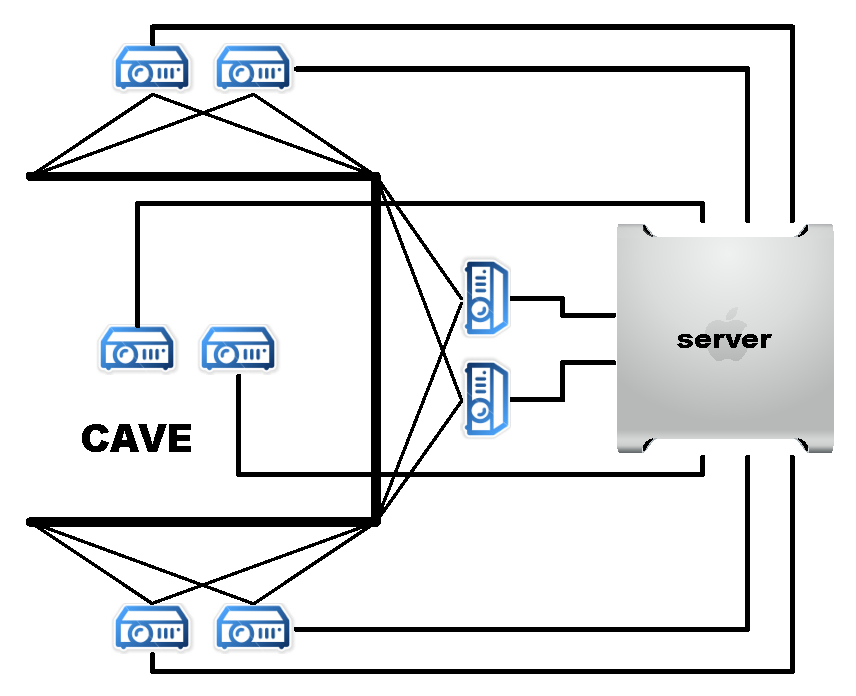
\includegraphics[width=0.5\textwidth]{../figures/1node_architecture}
	\caption{Resources for Setup with a single workstation with four graphics cards (2 pipes per card)}
	\label{fig:1nodeSetup}
\end{figure}

Figure \ref{fig:1nodeConfig} shows a graphical representation of the configuration. 
\begin{figure}[H]
	\centering
	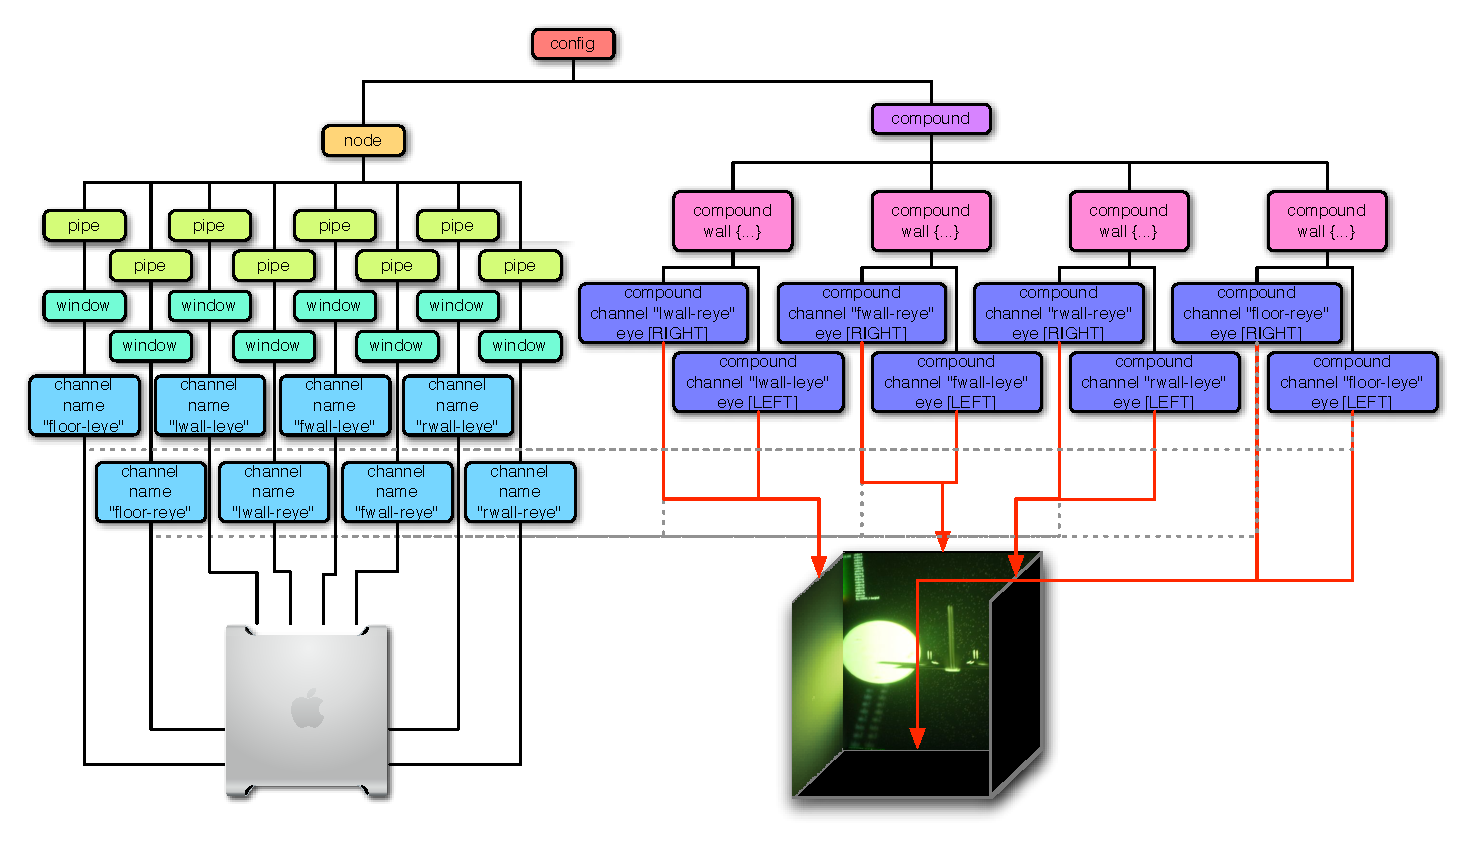
\includegraphics[width=1\textwidth]{../figures/1nodeConfig}
	\caption{Graphical representation of a single node config with a 4-sided CAVE as visualisation system}
	\label{fig:1nodeConfig}
\end{figure}

As shown in figure \ref{fig:1nodeConfig}, there are two pipes per graphics card. This is due to the fact that each graphics card has two outputs, each connected to a projector. Although, Equalizer allows the usage of multiple channels within a single window. This should not be used in combination with the \gls{cave} Rendering Framework.

An example configuration file for this setup can be found in Appendix \nameref{app:1nodeConfig}.

\subsection{six-node setup}
The second setup consists of six separate nodes, each connected to one projector. The setup is illustrated in Figure \ref{fig:6nodeSetup}.
\begin{figure}[H]
	\centering
	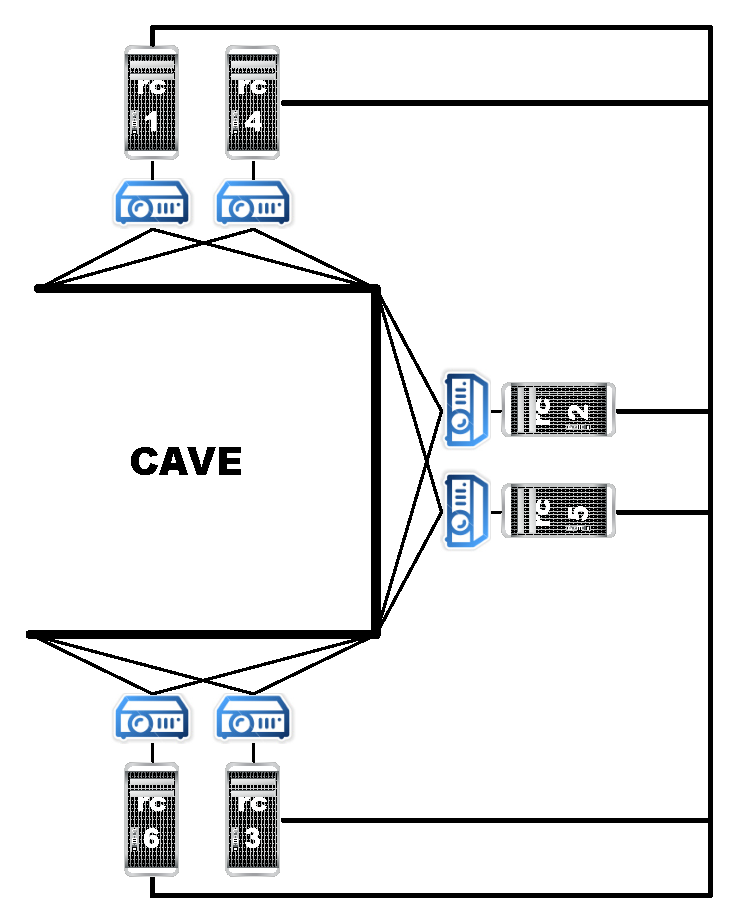
\includegraphics[width=0.5\textwidth]{../figures/6node_architecture}
	\caption{Resources for Setup with 6 connected workstations}
	\label{fig:6nodeSetup}
\end{figure}

Figure \ref{fig:6nodeConfig} shows a graphical representation of the configuration. 
\begin{figure}[H]
	\centering
	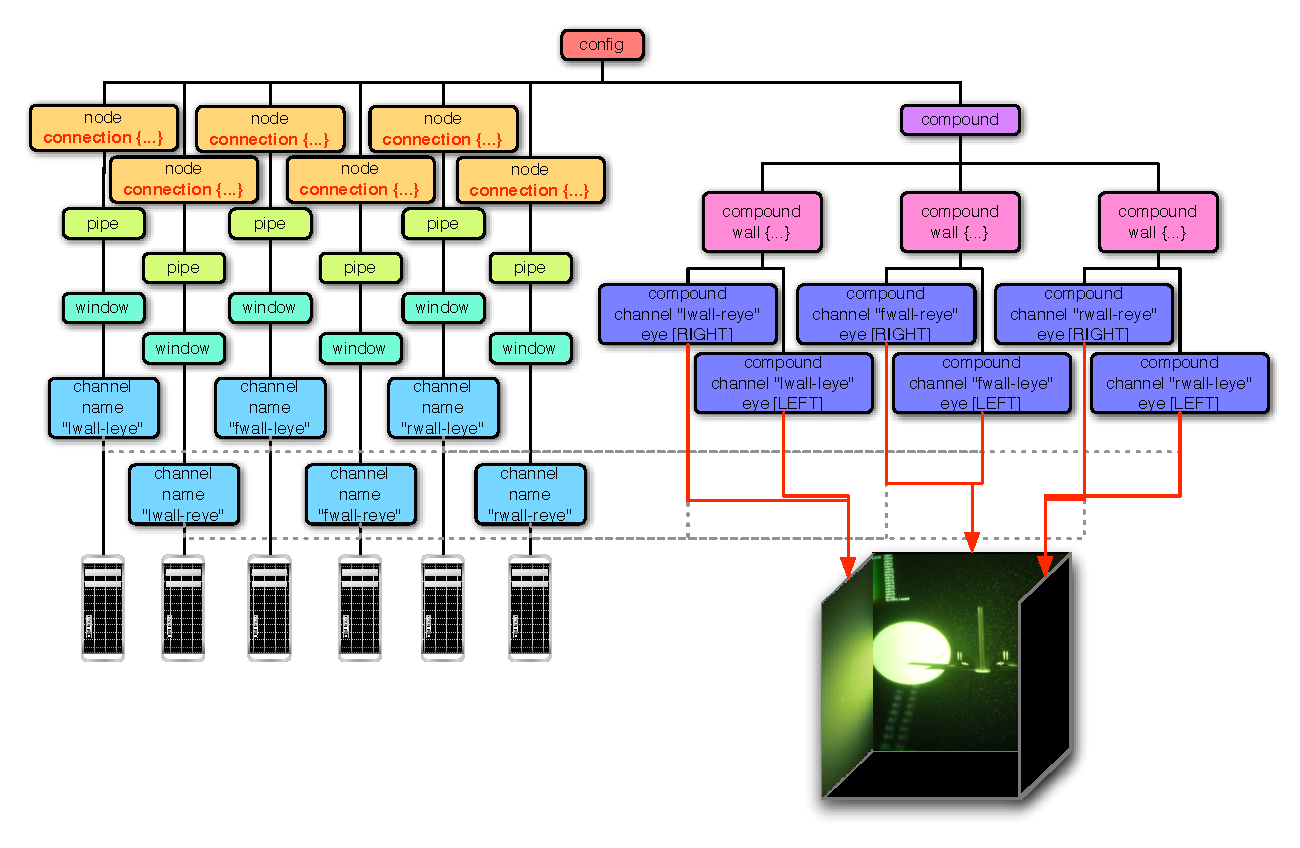
\includegraphics[width=1.0\textwidth]{../figures/6nodeConfig}
	\caption{Graphical representation of a 6-node config with a 3-sided CAVE as visualisation system}
	\label{fig:6nodeConfig}
\end{figure}

As shown in the figure \ref{fig:6nodeConfig}, each node has its own pipe (\gls{gpu} representation). To connect the nodes, each node has to contain a \texttt{connection} section with at least its hostname or IP address. Furthermore, one of the hosts acts as the server, which hast to be accessible by all other nodes via \gls{ssh}; Preferably without password verification. Further information concerning the authentication between hosts can be found in the \emph{User Manual}.

An example configuration file for this setup can be found in Appendix \nameref{app:6nodeConfig}.

